\section{Prototype Zero}
After gathering information from user questionnaires, conducting a competitor analysis, and creating tasks and dialogues using the methods described earlier, we moved on to developing the first prototype of our application interface. We used a tool called Justinmind, which allowed us to build the prototype by defining various windows, their connections, and the overall look and feel of the application. This tool helped us create a simple, clear, but accurate representation of our idea and its functionalities.
In the rest of the chapter, we are going to illustrate the prototype, dividing it by its different functionalities. This walkthrough will show how each feature is designed to meet user needs and contribute to the overall user experience.
	\subsection{Add document from saved file}

		\begin{figure}[htbp]
			\centering
			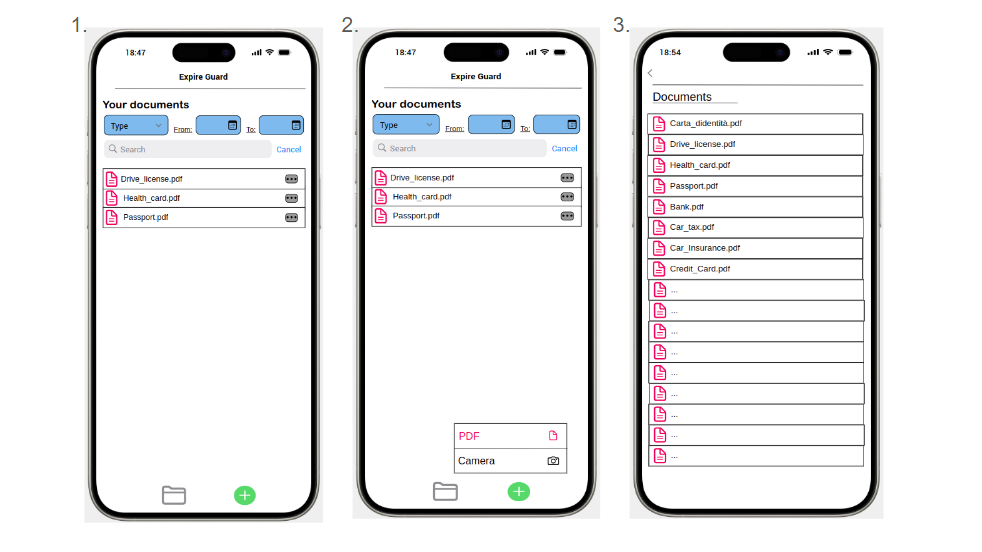
\includegraphics[width=0.9\textwidth]{../mockups/add_doc_pdf_1.png}  % Replace 'example-image' with the filename of your image
		\end{figure}
		
		\begin{figure}[htbp]
			\centering
			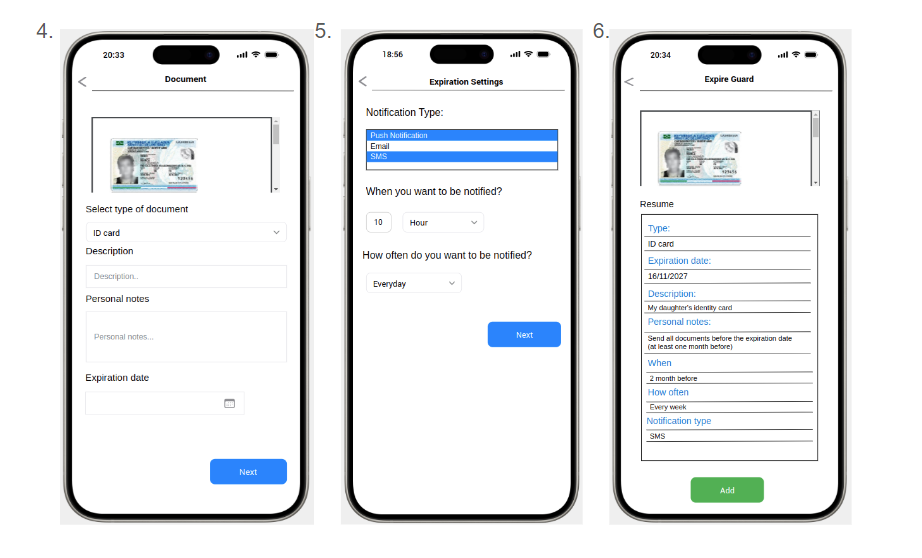
\includegraphics[width=0.85\textwidth]{../mockups/add_doc_pdf_2.png}  % Replace 'example-image' with the filename of your image
		\end{figure}
		\clearpage
	\subsection{Add document using camera scan}

		\begin{figure}[htbp]
			\centering
			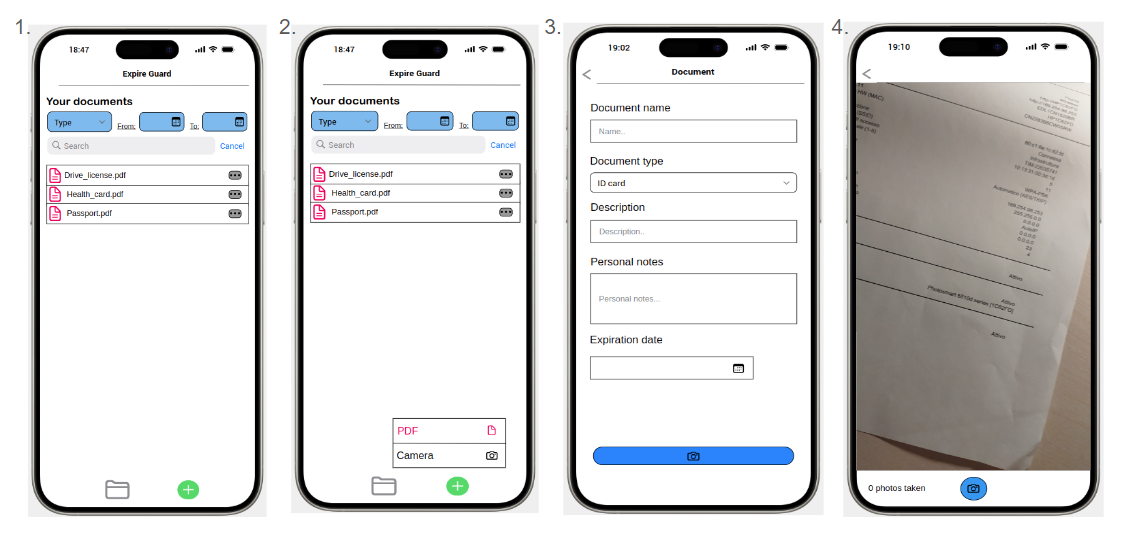
\includegraphics[width=0.9\textwidth]{../mockups/add_doc_cam_1.png}  % Replace 'example-image' with the filename of your image
		\end{figure}

		\begin{figure}[htbp]
			\centering
			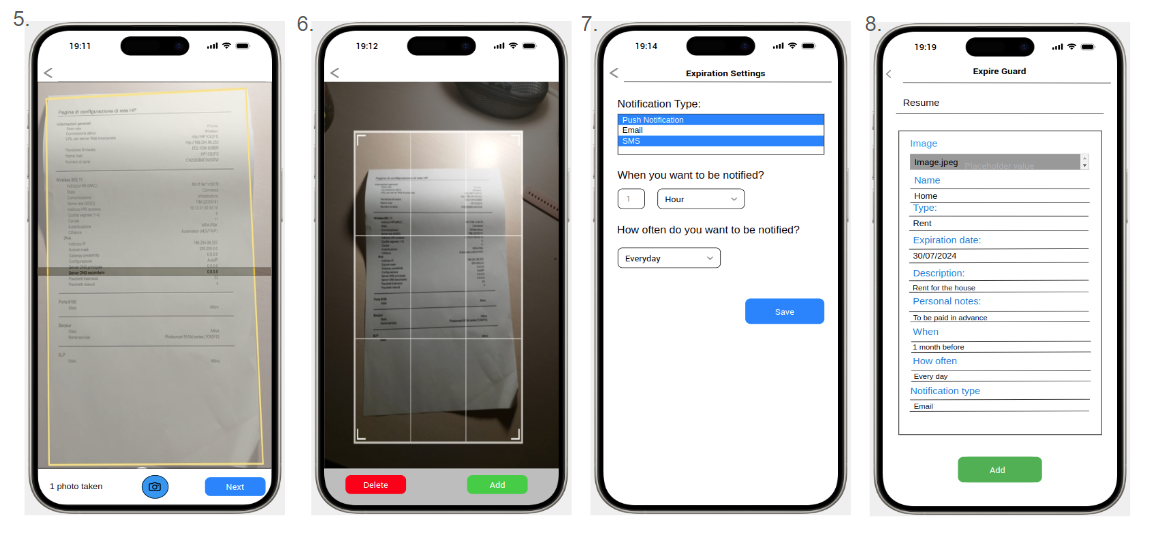
\includegraphics[width=0.9\textwidth]{../mockups/add_doc_cam_2.png}  % Replace 'example-image' with the filename of your image
		\end{figure}
		\clearpage
	\subsection{View document}
		
		\begin{figure}[htbp]
			\centering
			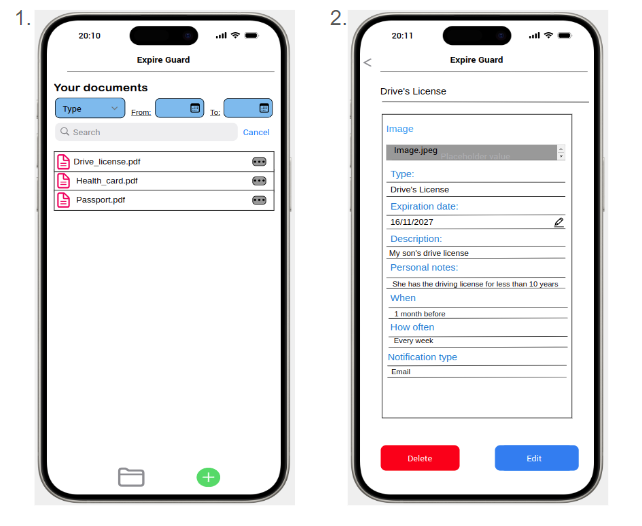
\includegraphics[width=0.7\textwidth]{../mockups/view_doc.png}  % Replace 'example-image' with the filename of your image
		\end{figure}
		\clearpage
	\subsection{Edit document description and personal notes}
		
		\begin{figure}[htbp]
			\centering
			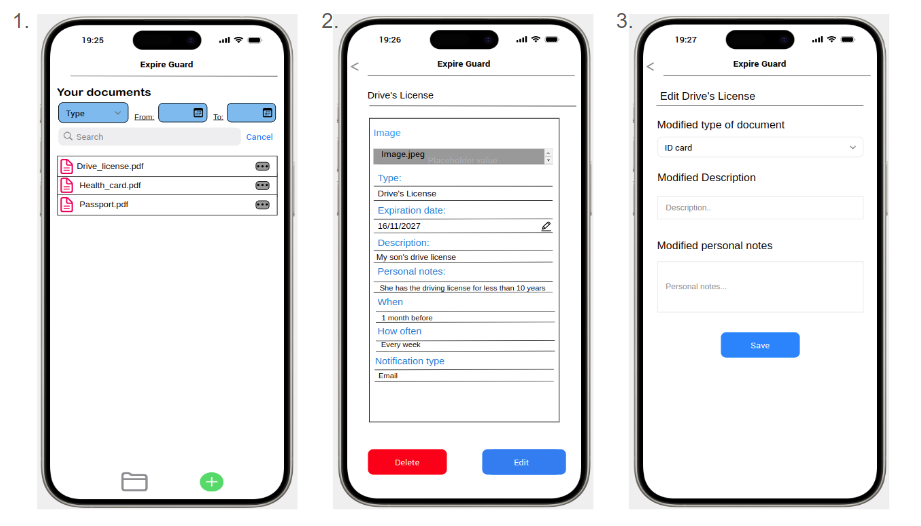
\includegraphics[width=0.9\textwidth]{../mockups/edit_doc_meta_1.png}  % Replace 'example-image' with the filename of your image
		\end{figure}
		\clearpage
	\subsection{Edit document Expiration date and Expiration Settings}

		\begin{figure}[htbp]
			\centering
			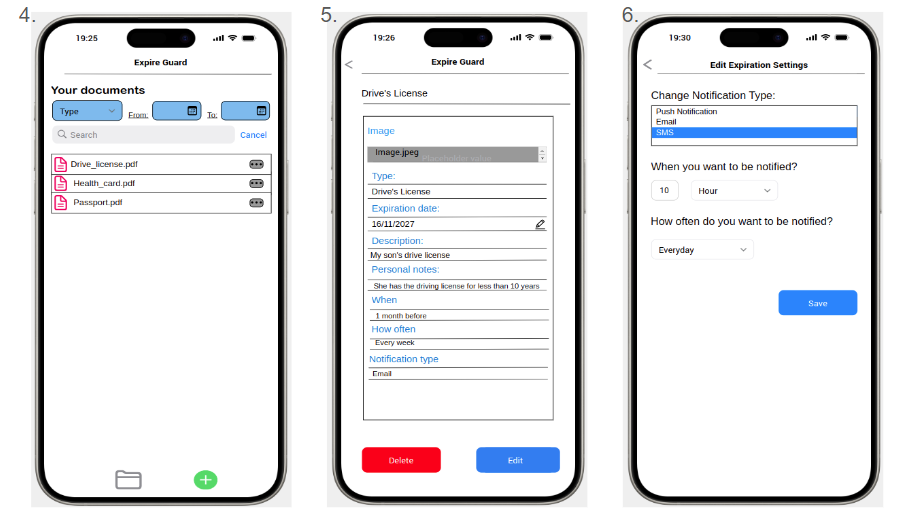
\includegraphics[width=0.9\textwidth]{../mockups/edit_doc_expr_1.png}  % Replace 'example-image' with the filename of your image
		\end{figure}
		\clearpage
	\subsection{Delete document}

		\begin{figure}[htbp]
			\centering
			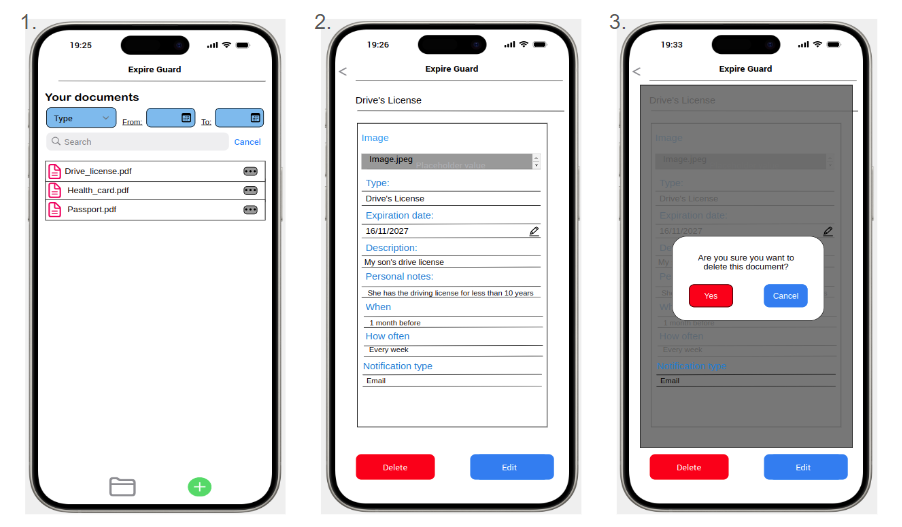
\includegraphics[width=0.9\textwidth]{../mockups/delete_doc.png}  % Replace 'example-image' with the filename of your image
		\end{figure}
		\clearpage
		
